\documentclass{article} % For LaTeX2e
\usepackage{cos424,times}
\usepackage{hyperref}
\usepackage{url}
\usepackage{graphicx}
\usepackage{amsmath}
\usepackage{multirow}
\usepackage{caption}
\usepackage{subcaption}

\bibliographystyle{plos2009}

\title{Spam Classification}

\author{Curtis Belmonte\\
{\tt\small curtislb@princeton.edu}
\and
Dorothy Chen\\
{\tt\small dschen@princeton.edu}
}

\newcommand{\fix}{\marginpar{FIX}}
\newcommand{\new}{\marginpar{NEW}}

\begin{document}

\maketitle

\begin{abstract}
Spam, or unsolicited email, is becoming an increasingly large problem as email becomes more and more popular. In this assignment, we discuss various machine learning methods and use them to create spam classifiers. We then analyze the results and effectiveness of these methods. 
\end{abstract}

%------------------------------------------------------------------------
\section{Introduction and background}
Email is something used daily by a large number of people. Advertisers and other people trying to sell things have taken advantage of this fact by sending out unsolicited emails, which is referred to as spam. In response to this, spam filters were created to identify these emails and to keep them from clogging up inboxes.

%------------------------------------------------------------------------
\section{Description of data and data processing}
The training data set consists of 22,500 spam emails and 22,500 non-spam emails from the trec07p data set. We used the provided script to define a vocabulary create a bag-of-words representation for each email. The resulting vocabulary contained 9579 words. The classifiers are built using these bag-of-words representations as features for the training data. The testing data set consists of 2,500 spam emails and 2,500 non-spam emails from the same corpus, and they are processed in a similar manner to also create bag-of-words representations. 

%------------------------------------------------------------------------
\section{Methods}
We used the methods implemented in the scikit-learn package. [1]
\subsection{Naive Bayes, using multinomial implementation}
As a baseline, we trained a Naive Bayes multinomial model on all of the training data using the default parameters provided by scikit-learn. The default parameters included Laplace smoothing, learning class prior probabilities, and no previously provided class priors. 

\subsection{Decision tree}
We also used the default parameters, which meant that splits were determined using Gini impurity, the best split at each node was chosen, and the depth of the tree was not constrained. However, nodes were only split if it contained at least two samples; a leaf could only exist if it had at least one sample. Because of the large number of features and because the depth of the tree was not constrained, this method was significantly slower than the other two. 

\subsection{Random forests with 10 trees}
We once again used the default parameters. This includes building 10 random trees using Gini impurity. This method constrains tree height when growing the tree. Because of this, random forests ran much more quickly than the decision tree.

%------------------------------------------------------------------------
\section{Results}
\subsection{Multinomial naive Bayes}
Using this classifier, we predicted labels for the testing data and got an accuracy rate of 98.74\%. The ROC curve can be seen in figure \ref{fig:roc}(a) and indicates a high true positive and low false positive rate.

\subsection{Decision tree}
Training this classifier on all available training data and testing on the provided testing set resulted in an accuracy rate of of 99.5\%. The ROC curve can be seen in figure \ref{fig:roc}(b). Like the ROC curve for naive Bayes, it indicates that this method has a high true positive and low false positive rate. This method's higher accuracy (relative to naive Bayes) is shown by the fact that the ROC curve is barely visible because it's almost entirely on top of the axis.

\subsection{Random forests}
Using this method, we got 99.58\% accuracy. The ROC curve can be seen in figure \ref{fig:roc}(c). This method, like the other two, has a very high true positive and low false positive rate. Like the ROC curve for the decision tree, this ROC curve is almost entirely on top of this axis. This indicates the high level of accuracy of this method. 

In an effort to view the data more clearly, we plotted the data on log scales. Specifically, we plotted the x-axis on a log10 scale in order to examine lower false positive rates. However, this did not significantly change the quality of the graph so we decided not to include it in this report. 

\begin{figure}[h]
  \centering
  \begin{subfigure}{0.45\textwidth}
    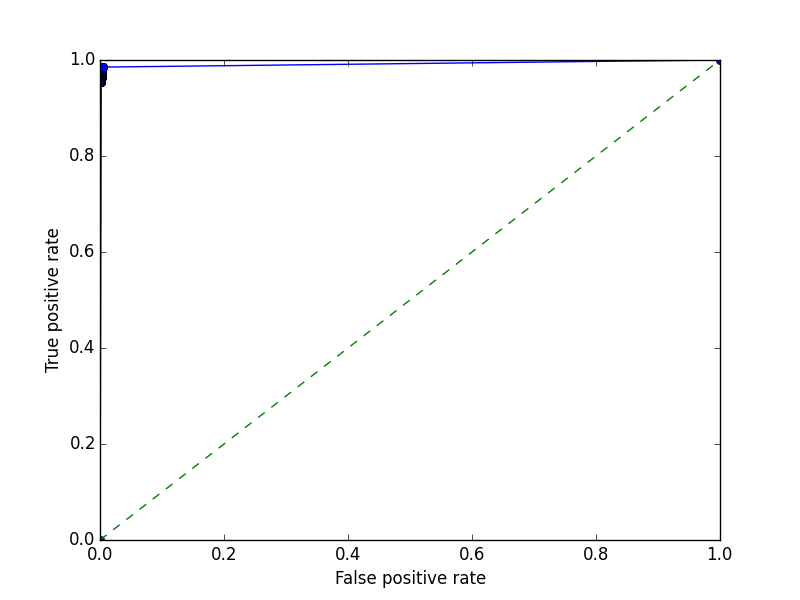
\includegraphics[width=\textwidth]{naive_bayes_roc_curve.png}
    \caption{Multinomial Naive Bayes}
  \end{subfigure}
  \begin{subfigure}{0.45\textwidth}
    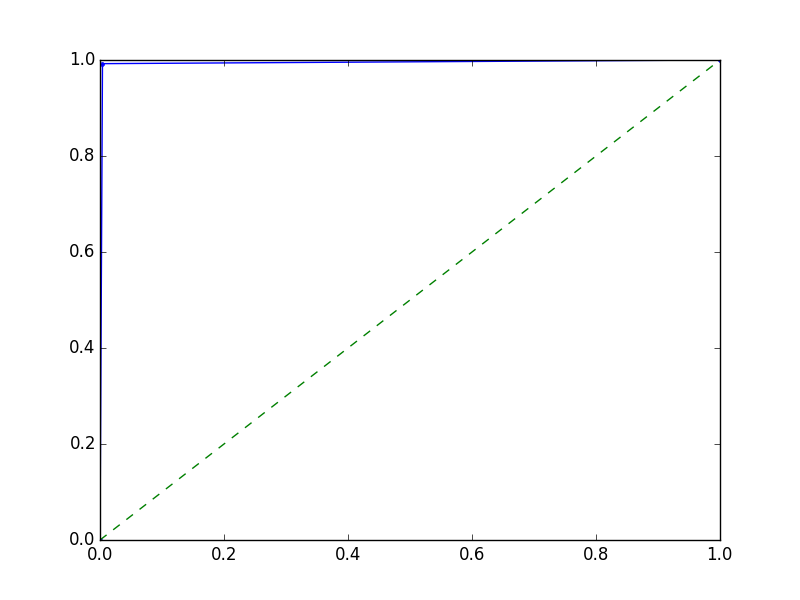
\includegraphics[width=\textwidth]{decision_tree_roc_curve.png}
    \caption{Decision Tree}
  \end{subfigure}
  \begin{subfigure}{0.45\textwidth}
    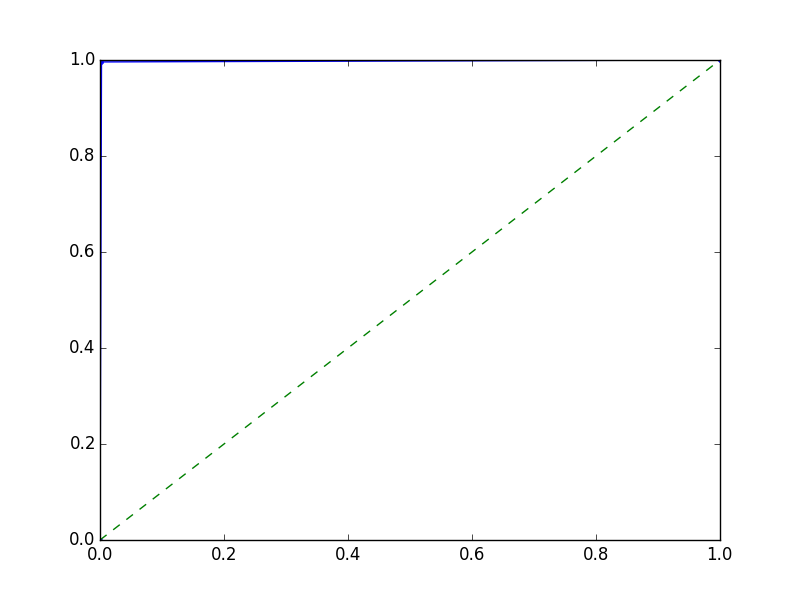
\includegraphics[width=\textwidth]{random_forest_roc_curve.png}
    \caption{Random Forest}
  \end{subfigure}
  \caption{ROC curves for various methods}
  \label{fig:roc}
\end{figure}

%------------------------------------------------------------------------
\section{Analysis of results}
\subsection{Initial results}
For each classification method, we used stratified 5-fold cross-validation. We wanted to use the same number of folds across all methods in order to facilitate comparison. Initially, we used a higher number but decided to reduce the number of folds due to time considerations when running decision tree. 

Preliminary comparison of results, described in the previous section, was done using accuracy and ROC curves. We then did further analysis and comparison using precision, recall, and F1-scores. In figure \ref{fig:table}, we can see values for the methods run on both the entire corpus at once and for averages from running 5-fold cross-validation. 

There are a few differences between running classifiers on the entire corpus versus doing cross-validation. The most easily explained of these is the time: because cross-validation trains using 4/5 of the available data, it will take less time than training on all the data. 

One thing to note is that for random forests, running time varies by around 1-1.5 seconds between runs. This is a significant amount, considering it takes around 7-9 seconds to run in total. This is most likely due to the fact that random forests selects a random subset of features to split on each time; some runs will get better features (that result more quickly in pure nodes) than others. 

Another notable result happened when running cross-validation using decision tree. We had one run that had 0.939 accuracy, 0.992 precision, 0.8870 recall, and 0.936 $F_1$. In comparison to our overall and averaged results, which can be found in figure \ref{fig:table}, these values (except for precision) are extremely low. 

\begin{figure}[h]
  \begin{tabular}[h]{ | c | c | r | r | r | r | r | }
    \hline
    Classifier    &                  & Time (s) & Accuracy & Precision & Recall & $F_1$  \\ \hline
    Naive Bayes   & Entire corpus    & 1.51     & 0.9874   & 0.9963    & 0.9784 & 0.9873 \\ \cline{2-7}
                  & Cross-validation & 1.25     & 0.9940   & 0.9984    & 0.9895 & 0.9939 \\ \hline
    Decision Tree & Entire corpus    & 150.0    & 0.9948   & 0.9950    & 0.9936 & 0.9947 \\ \cline{2-7}
                  & Cross-validation & 106.05   & 0.9856   & 0.9956    & 0.9752 & 0.9850 \\ \hline
    Random Forest & Entire corpus    & 11.46    & 0.9968   & 0.9992    & 0.9944 & 0.9968 \\ \cline{2-7}
                  & Cross-validation & 8.18     & 0.9976   & 0.9969    & 0.9984 & 0.9976 \\ \hline
  \end{tabular}
  \caption{Results from using various methods}
  \label{fig:table}
\end{figure}

\subsection{Running time}
As we can see in figure \ref{fig:table}, using Naive Bayes is by far the fastest of the three methods we used. Random forests are second fastest and still reasonably quick. Decision trees, however, are by far the slowest. This is due to the fact that we did not constrain the height of the tree 

\subsection{Feature selection}
We tried selection 5, 10, and 15\% of features. Performance among the three was best at the 5\% level of selection; we have included these results in figure \ref{fig:table_selected}. In comparison to training on the entire corpus, performance on the feature selected set in terms of accuracy, precision, recall, and $F_1$ decreased. On the other hand, running time also decreased dramatically. Therefore, feature selection presents a tradeoff between correctness and computational time: in time-sensitive situations, using feature selection would definitely be preferable. 

Because the drop in correctness is most likely not as significant as the boost in performance time-wise in most situations, feature-selected training and testing is probably preferable. In situations that require high accuracy/precision, however, using the full feature set would still be better. 

\begin{figure}[h]
  \begin{tabular}[h]{ | c | c | r | r | r | r | r | }
    \hline
    Classifier    &                  & Time (s) & Accuracy & Precision & Recall & $F_1$  \\ \hline
    Naive Bayes   & Entire corpus    & 0.08     & 0.9526   & 0.9752    & 0.9288 & 0.9514 \\ \cline{2-7}
                  & Cross-validation & 0.07     & 0.9629   & 0.9636    & 0.9632 & 0.9630 \\ \hline
    Decision Tree & Entire corpus    & 2.96     & 0.9936   & 0.9952    & 0.9920 & 0.9936 \\ \cline{2-7}
                  & Cross-validation & 2.19     & 0.9925   & 0.9956    & 0.9894 & 0.9925 \\ \hline
    Random Forest & Entire corpus    & 0.82     & 0.9972   & 0.9984    & 0.9960 & 0.9972 \\ \cline{2-7}
                  & Cross-validation & 0.60     & 0.9976   & 0.9972    & 0.9981 & 0.9976 \\ \hline
  \end{tabular}
  \caption{Results from using various methods after performing feature selection}
  \label{fig:table_selected}
\end{figure}

%------------------------------------------------------------------------
\section{Conclusion and possible extensions}

We feel that using a different model to represent the emails' content would be an interesting and potentially useful extension. While the bag-of-words model was certainly effective, many features were lost; in particular, we feel that things such as word order, capitalization, and punctuation are especially important in language and that their exclusion may have negatively impacted performance. 

To elaborate on the above points, word order is important because it encodes meaning and context of sentences--single words on their own may be ambiguous. Capitalization also matters, as emails in all capitals, for example, are probably more likely to be spam. Punctuation also matters, because emails with punctuation are more likely to have proper grammar, and correct grammar intuitively seems indicative of non-spam (or, at least non-computer generated) emails. 

Another possible extension is using a different data set. While our classifier performed very well on this particular data set, that performance might not necessarily hold for use on other data sets. This is because the set itself might have some trait that's highly indicative of spam versus not-spam that is not indicative of or present in the population of emails as a whole. It would be helpful to use a classifier trained on one set to test a different email corpus. 

%------------------------------------------------------------------------
\section{Acknowledgments}

%------------------------------------------------------------------------
\section{References}
\bibliography{ref}
[1] http://scikit-learn.org/stable/

\end{document}
